\documentclass{TDP005mall}

\usepackage{graphicx}
\usepackage{float}

\newcommand{\version}{Version 1.0}
\author{Albin Dahlén, \url{albda746@student.liu.se}\\
  Filip Ingvarsson, \url{filin764@student.liu.se}}
\title{Designspecifikation}
\date{2022-11-21}
\rhead{Albin Dahlén\\
Filip Ingvarsson}


\begin{document}
\projectpage
\section{Revisionshistorik}
\begin{table}[!h]
\begin{tabularx}{\linewidth}{|l|X|l|}
\hline
Ver. & Revisionsbeskrivning & Datum \\\hline
1.0 & Första utkast & 22-11-25 \\\hline
\end{tabularx}
\end{table}

\section{Detaljbeskrivning av Player}
Syftet med Playerklassen är att representera den entitet som spelaren kontrollerar.

Playerklassen bör interagera med projectile klassen då spelaren ska skapa en projektil när hen skjuter.
Playerklassen bör även interagera med Enemy klassen för att ta reda på om spelaren kolliderat med en fiende och i så fall ska spelarens hälska minska.
Slutligen bör playerklassen även interagera med Obstacleklassen för att ta reda på om vi kolliderat med ett hinder.

\section{Detaljbeskrivning av Gamestate}
Gamestate är ett av tillstånden som vårt program kommer kunna vara i, den har även förmågan att ändra tillstånd till "menystate" och "endstate" som är ett meny tillstånd respektive
ett tillstånd precis innan spelet ska avslutas.

När spelet är i Gamestate är då som spelet spelas och behöver således samarbeta med Gameklassen för att kunna spela, pausa eller avsluta spelet.


\section{Klassdiagram}


\begin{figure}[!h]
  \begin{center}
  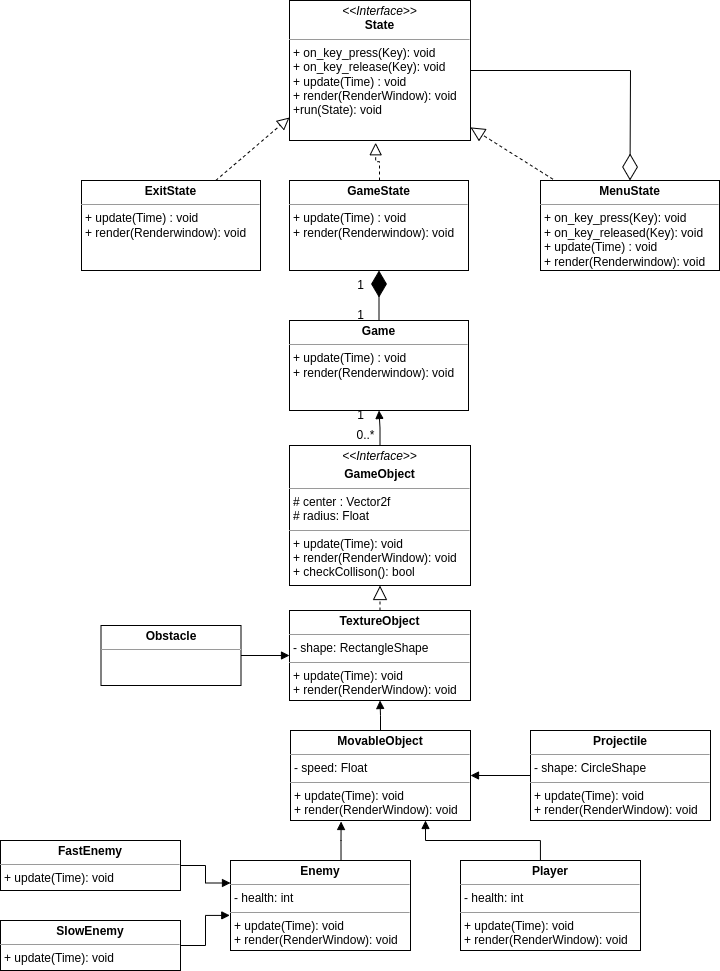
\includegraphics[width=0.95\linewidth]{uml.png}
  \caption {UML-diagram på designen}
  \label {fig:picture}
  \end{center}
\end {figure}


\end{document}
